\section{Basics of Wireless Communication}

\subsection{Basics}

\begin{minipage}{\linewidth}
    \centering      
    \def\svgwidth{\columnwidth}
    %% Creator: Inkscape 1.0 (4035a4fb49, 2020-05-01), www.inkscape.org
%% PDF/EPS/PS + LaTeX output extension by Johan Engelen, 2010
%% Accompanies image file 'L1_wireless_system.pdf' (pdf, eps, ps)
%%
%% To include the image in your LaTeX document, write
%%   \input{<filename>.pdf_tex}
%%  instead of
%%   \includegraphics{<filename>.pdf}
%% To scale the image, write
%%   \def\svgwidth{<desired width>}
%%   \input{<filename>.pdf_tex}
%%  instead of
%%   \includegraphics[width=<desired width>]{<filename>.pdf}
%%
%% Images with a different path to the parent latex file can
%% be accessed with the `import' package (which may need to be
%% installed) using
%%   \usepackage{import}
%% in the preamble, and then including the image with
%%   \import{<path to file>}{<filename>.pdf_tex}
%% Alternatively, one can specify
%%   \graphicspath{{<path to file>/}}
%% 
%% For more information, please see info/svg-inkscape on CTAN:
%%   http://tug.ctan.org/tex-archive/info/svg-inkscape
%%
\begingroup%
  \makeatletter%
  \providecommand\color[2][]{%
    \errmessage{(Inkscape) Color is used for the text in Inkscape, but the package 'color.sty' is not loaded}%
    \renewcommand\color[2][]{}%
  }%
  \providecommand\transparent[1]{%
    \errmessage{(Inkscape) Transparency is used (non-zero) for the text in Inkscape, but the package 'transparent.sty' is not loaded}%
    \renewcommand\transparent[1]{}%
  }%
  \providecommand\rotatebox[2]{#2}%
  \newcommand*\fsize{\dimexpr\f@size pt\relax}%
  \newcommand*\lineheight[1]{\fontsize{\fsize}{#1\fsize}\selectfont}%
  \ifx\svgwidth\undefined%
    \setlength{\unitlength}{1164.91748047bp}%
    \ifx\svgscale\undefined%
      \relax%
    \else%
      \setlength{\unitlength}{\unitlength * \real{\svgscale}}%
    \fi%
  \else%
    \setlength{\unitlength}{\svgwidth}%
  \fi%
  \global\let\svgwidth\undefined%
  \global\let\svgscale\undefined%
  \makeatother%
  \begin{picture}(1,0.55304965)%
    \lineheight{1}%
    \setlength\tabcolsep{0pt}%
    \put(0,0){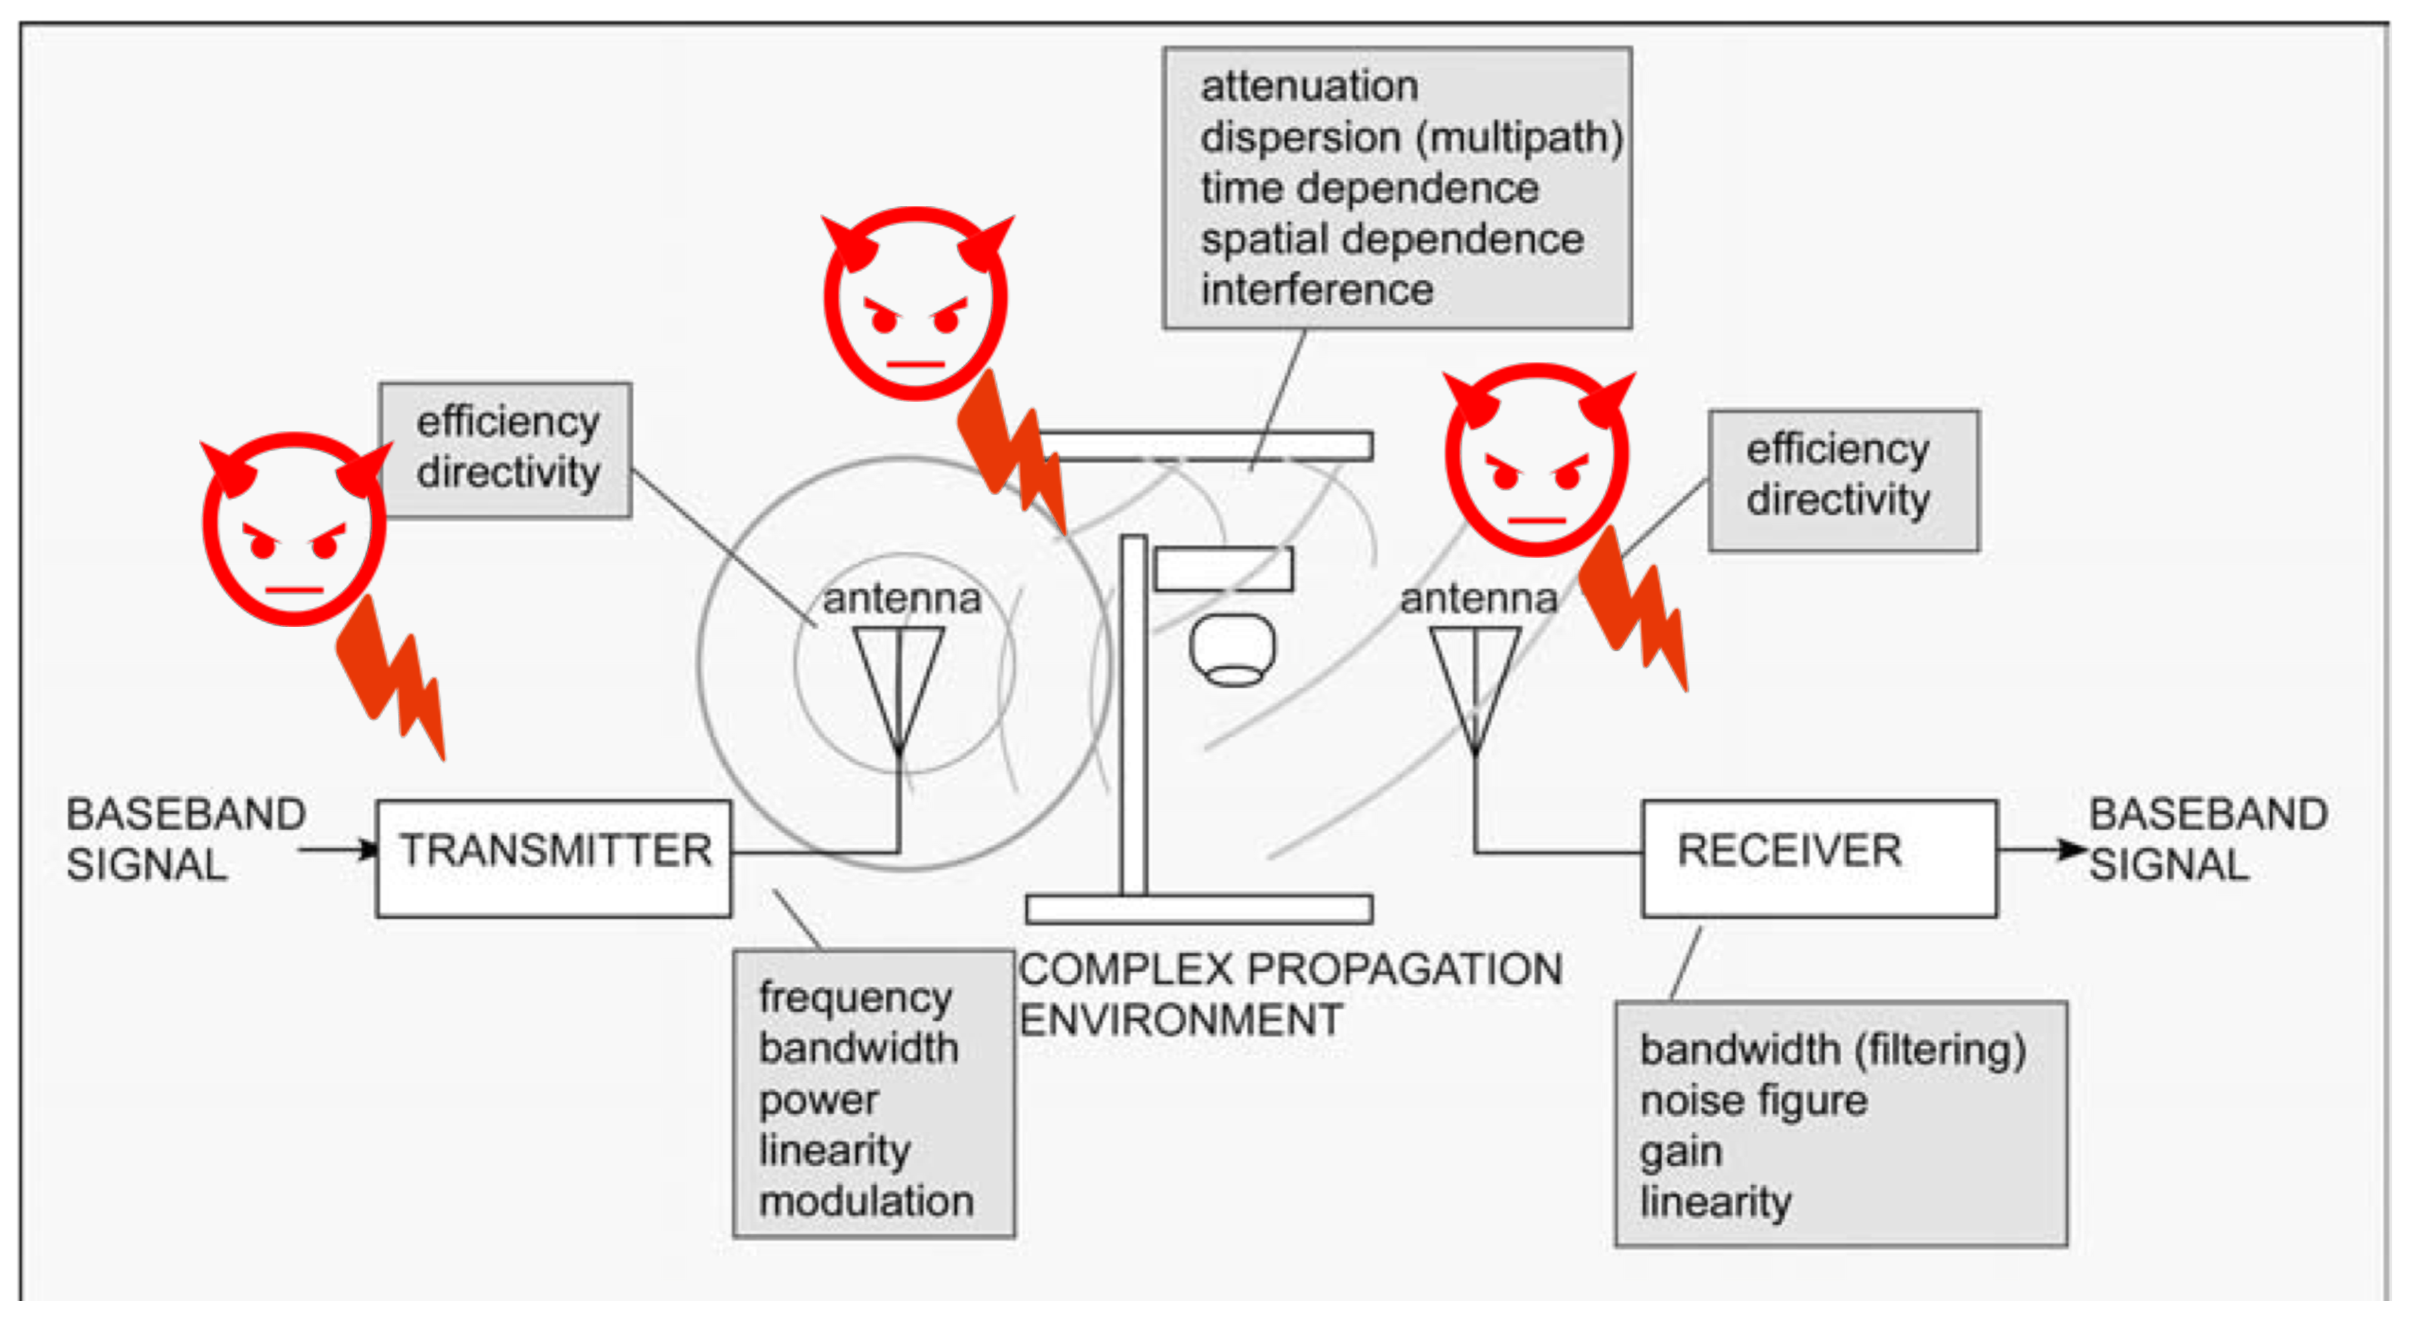
\includegraphics[width=\unitlength,page=1]{L1_wireless_system.pdf}}%
  \end{picture}%
\endgroup%
\end{minipage}

\paragraph{Radio Frequency Signal (RF):}
\begin{itemize}
    \item Communication using EM radiation waves at frq 3kHz-300GHz.
    \item Waves created by alternating current at desired communicatino frequency.
    \item \textcolor{orange}{$s(t) = A cos(2\pi ft + \phi)$} 
    \item f=frequency (Hz), A=Amplitude, t=time, $\phi$=phase, $\lambda$=wavelength=$c/f$, T=period=$1/f$.
    \item Inverse-square law wrt the distance from the source $p$ proportional to $17d`^2$
\end{itemize}


\paragraph{Modulation:} Signal modulation changes a sine wave to encode information. Different modulation techniques will require different bandwidths for the same data rate.
\begin{itemize}
    \item Binary Phase Shift Keying (BPSK)
    \item Amplitude Shift Keying (ASK)
\end{itemize}

\paragraph{Bandwidth:}Bandwidth can be imagined as a frequency width, sort of the fatness of the signal. What is the bandwidth of the modulated signal? It is still the same. The modulated signal takes on the bandwidth of the information signal it is carrying.

\paragraph{Baseband Signal:} Actual Information message you want to transmit.s

\paragraph{I/Q Signal representation:} Precisely varying the phase of a high frequency carrier sine wave in a hardware circuit according to an input message signal is difficult. Modulated information signal, that is not upmixed to carrier frequency yet (I/Q Data). A simple way of representing amplitude an phase of a signal.

\paragraph{RF Upconverter:} generates the carrier signal with amplitude and phase from I/Q data and returns the RF signal.

\paragraph{Frequency and Bandwidth of a Signal:} Bandwidth = measure of frequency content of the signal\\
\begin{minipage}{\linewidth}
    \centering      
    \def\svgwidth{\columnwidth}
    %% Creator: Inkscape 1.0 (4035a4fb49, 2020-05-01), www.inkscape.org
%% PDF/EPS/PS + LaTeX output extension by Johan Engelen, 2010
%% Accompanies image file 'L1_bandwidth.pdf' (pdf, eps, ps)
%%
%% To include the image in your LaTeX document, write
%%   \input{<filename>.pdf_tex}
%%  instead of
%%   \includegraphics{<filename>.pdf}
%% To scale the image, write
%%   \def\svgwidth{<desired width>}
%%   \input{<filename>.pdf_tex}
%%  instead of
%%   \includegraphics[width=<desired width>]{<filename>.pdf}
%%
%% Images with a different path to the parent latex file can
%% be accessed with the `import' package (which may need to be
%% installed) using
%%   \usepackage{import}
%% in the preamble, and then including the image with
%%   \import{<path to file>}{<filename>.pdf_tex}
%% Alternatively, one can specify
%%   \graphicspath{{<path to file>/}}
%% 
%% For more information, please see info/svg-inkscape on CTAN:
%%   http://tug.ctan.org/tex-archive/info/svg-inkscape
%%
\begingroup%
  \makeatletter%
  \providecommand\color[2][]{%
    \errmessage{(Inkscape) Color is used for the text in Inkscape, but the package 'color.sty' is not loaded}%
    \renewcommand\color[2][]{}%
  }%
  \providecommand\transparent[1]{%
    \errmessage{(Inkscape) Transparency is used (non-zero) for the text in Inkscape, but the package 'transparent.sty' is not loaded}%
    \renewcommand\transparent[1]{}%
  }%
  \providecommand\rotatebox[2]{#2}%
  \newcommand*\fsize{\dimexpr\f@size pt\relax}%
  \newcommand*\lineheight[1]{\fontsize{\fsize}{#1\fsize}\selectfont}%
  \ifx\svgwidth\undefined%
    \setlength{\unitlength}{1920bp}%
    \ifx\svgscale\undefined%
      \relax%
    \else%
      \setlength{\unitlength}{\unitlength * \real{\svgscale}}%
    \fi%
  \else%
    \setlength{\unitlength}{\svgwidth}%
  \fi%
  \global\let\svgwidth\undefined%
  \global\let\svgscale\undefined%
  \makeatother%
  \begin{picture}(1,0.5625)%
    \lineheight{1}%
    \setlength\tabcolsep{0pt}%
    \put(0,0){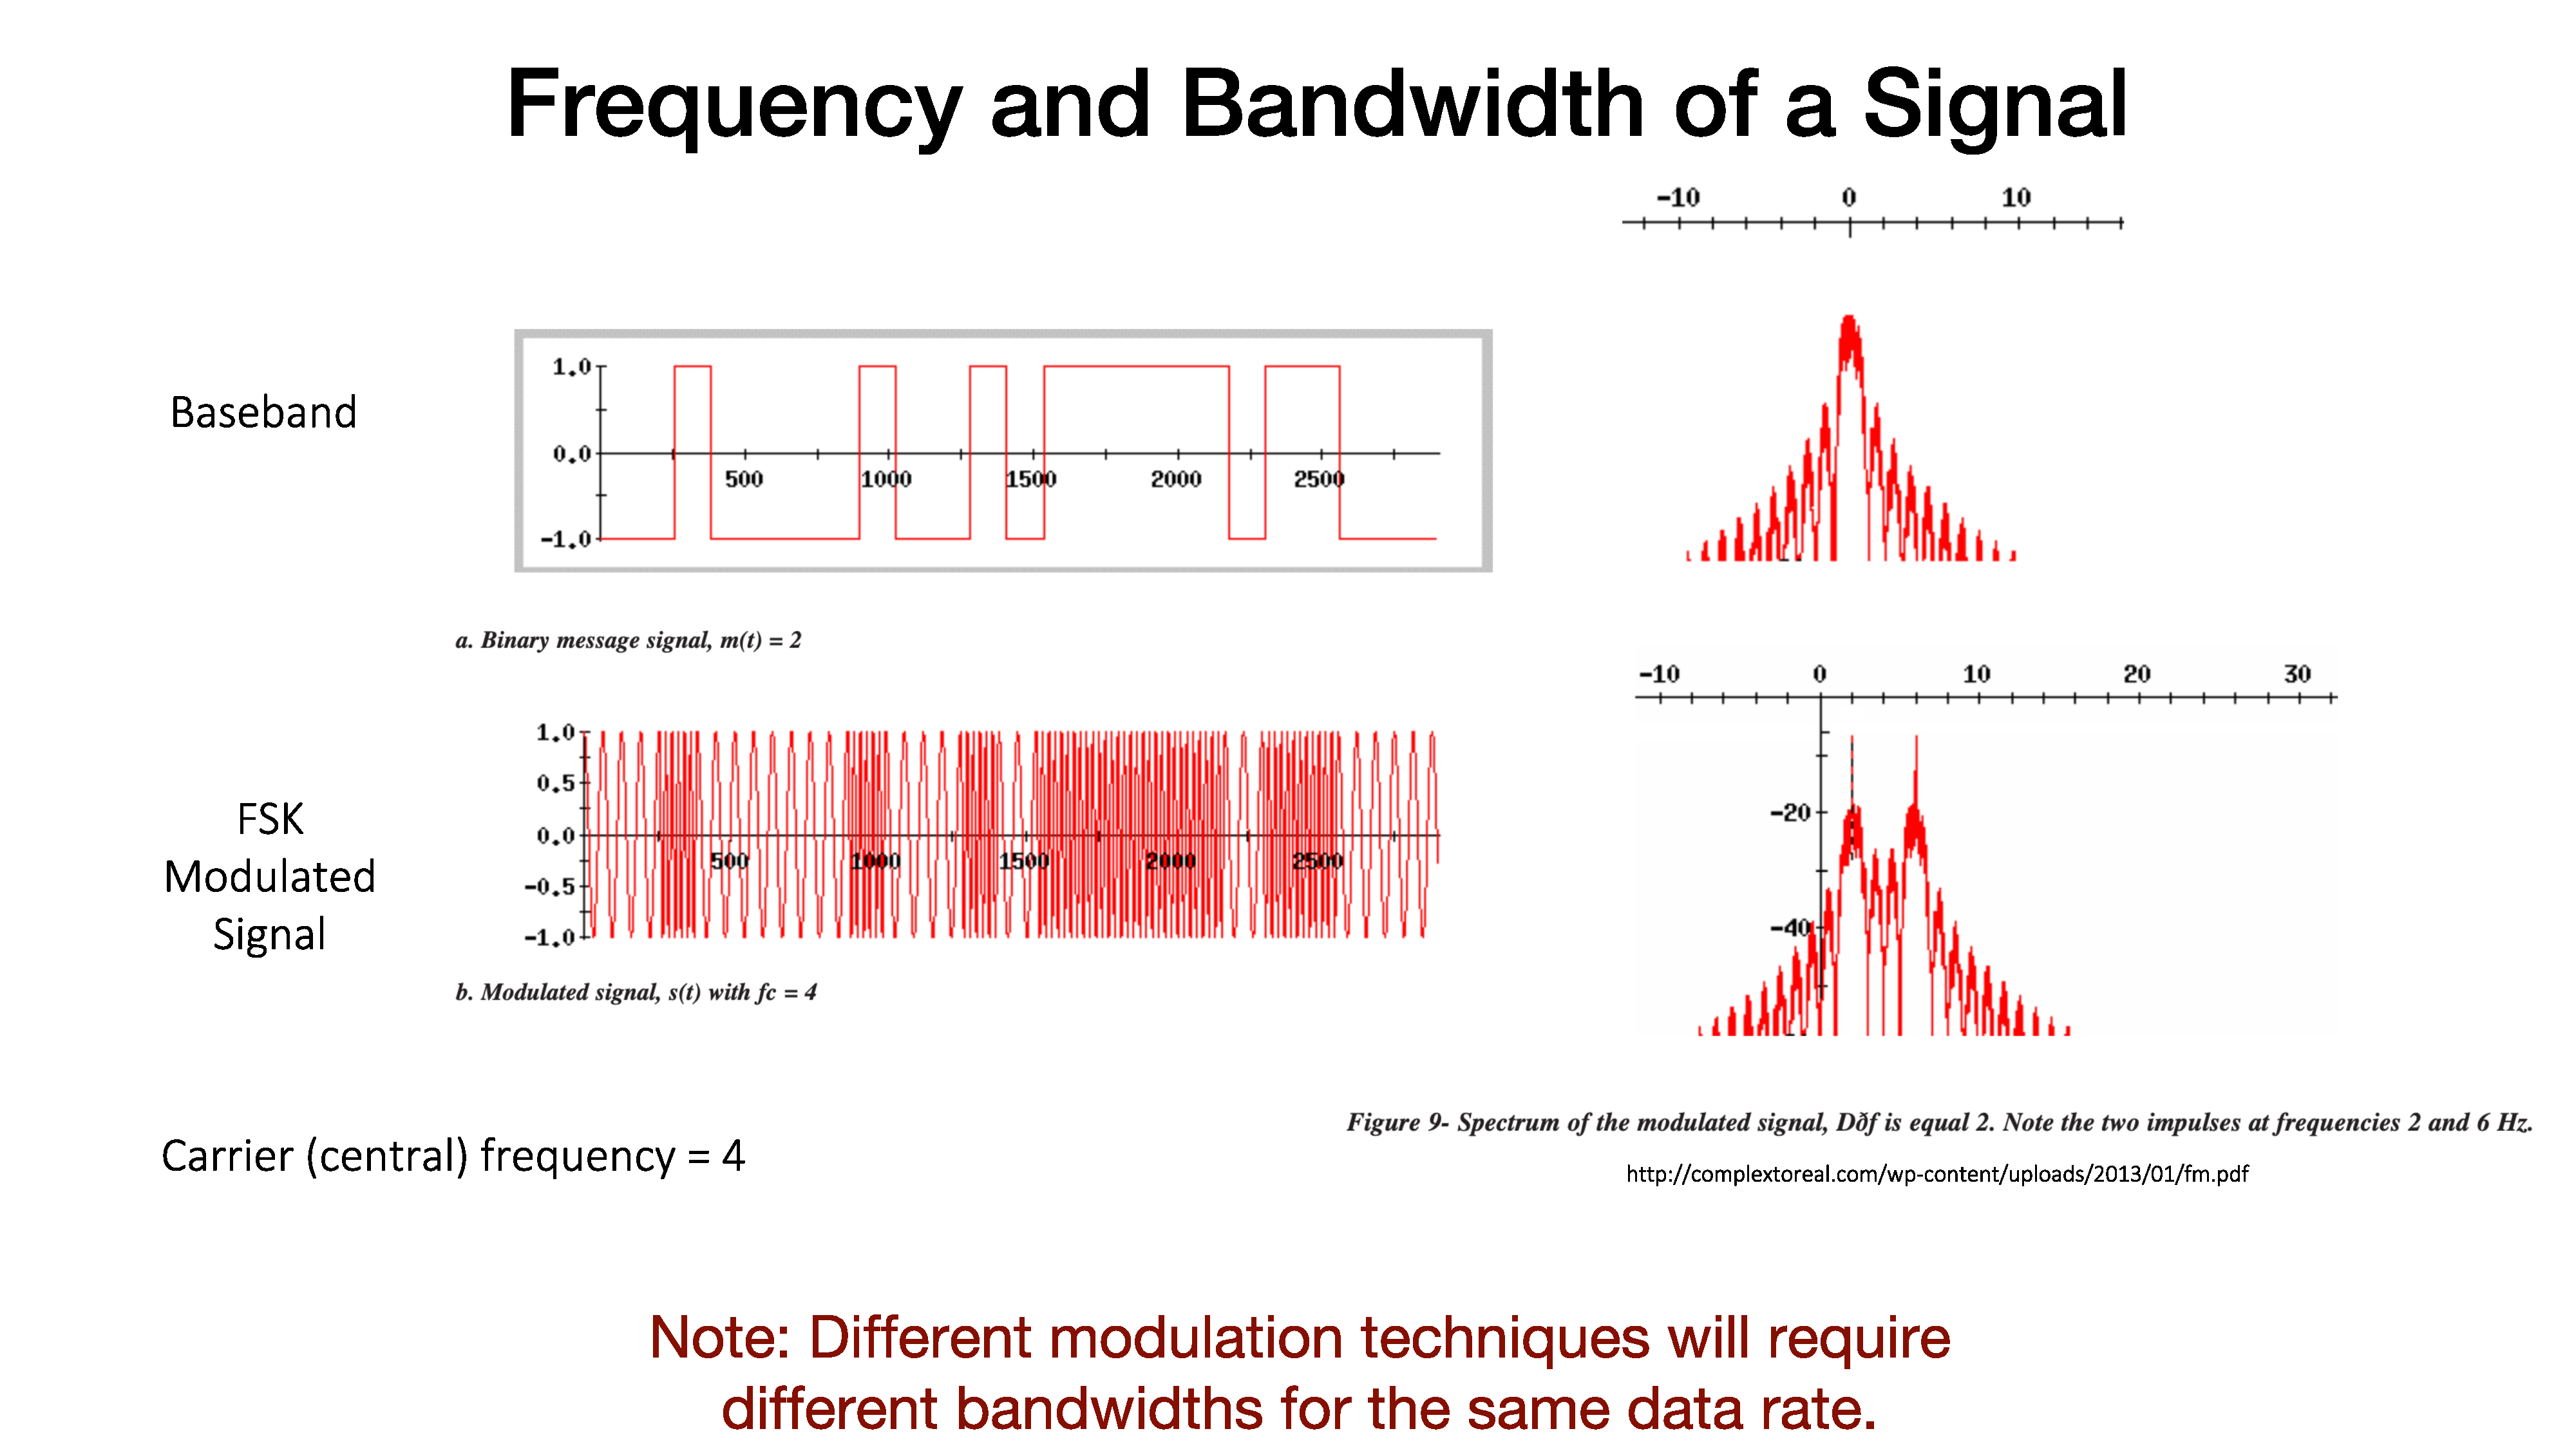
\includegraphics[width=\unitlength,page=1]{Figures/L1_bandwidth.pdf}}%
  \end{picture}%
\endgroup%
\end{minipage}

\begin{minipage}{\linewidth}
    \centering      
    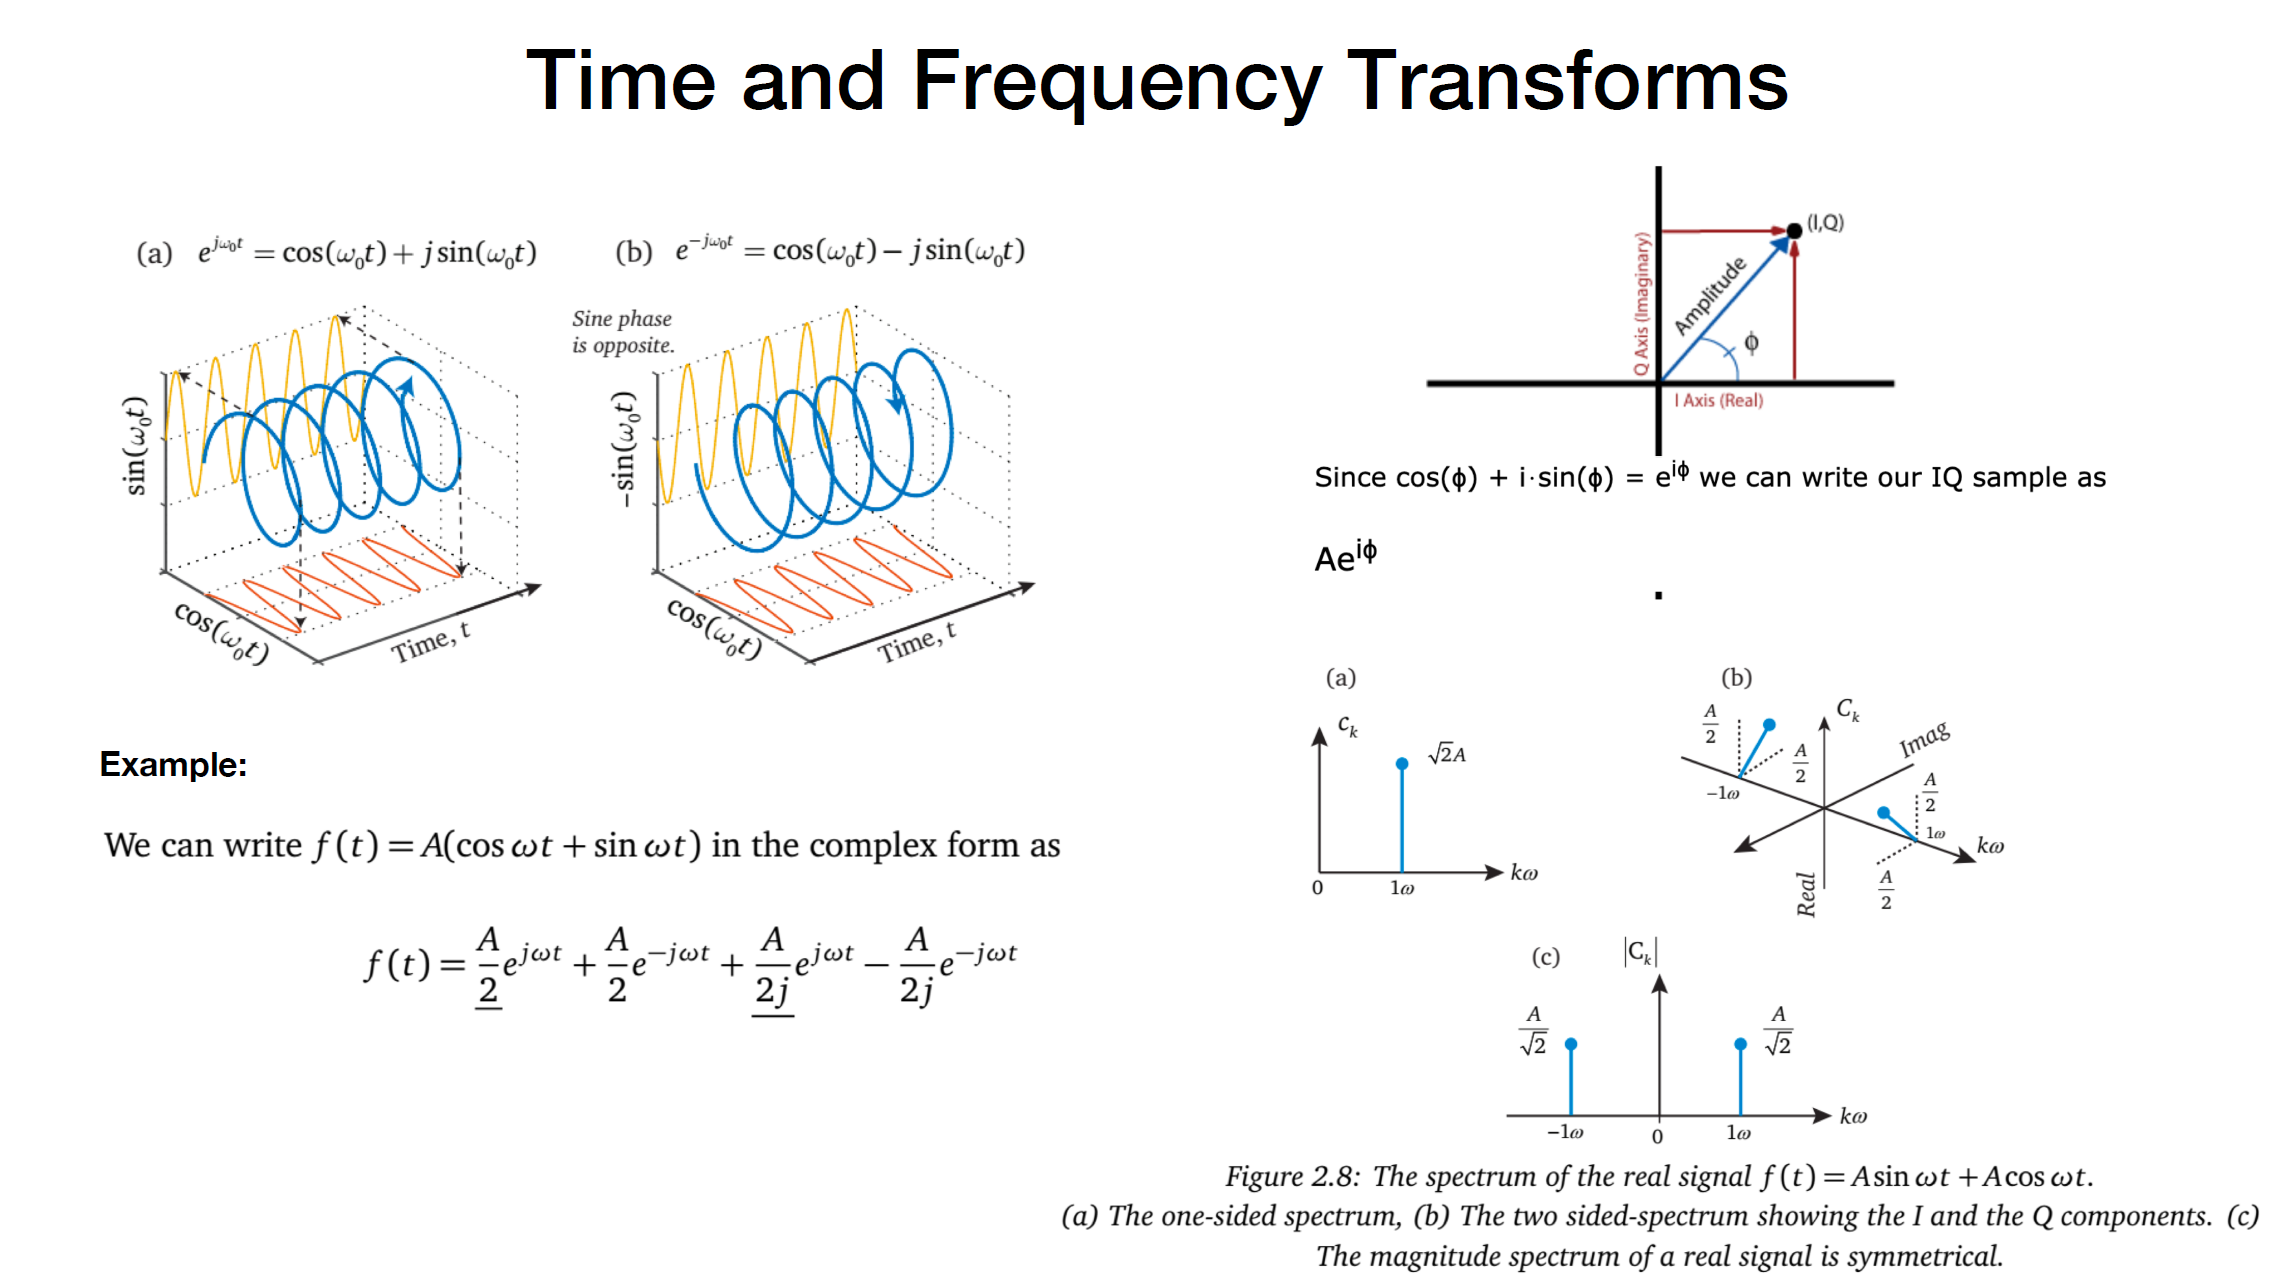
\includegraphics[width=\linewidth]{Figures/L1_frequency_transforms.PNG}
\end{minipage}

\paragraph{Antennas and Propagation:}
\begin{itemize}
    \item Tradeoff: Antenna Gain vs Beamwidth
    \item Beam steering antennas: Phase of the signal to each antenna is adjusted such that all the signals will be in phase, when viewed from a certain direction. Can steer the antenna array to transmit signals or receive signals from specific direction. (example applications Mimo, selective target jamming)
\end{itemize}

\paragraph{Transmitter Architecture: }
Key Properties are Transmitted power, carrier frequency, information bandwidth, modulation type.

\paragraph{Receiver Architecture: }
\begin{itemize}
    \item Key Properties: Receiver sensitivity (depends on the antenna, low noise amplifier, mixer)
    \item Software Defined Receivers SDR: low-cost, traditional components (such as mixers, amplifiers, modulators implemented in software), signal processed in PC.
\end{itemize}

\begin{minipage}{\linewidth}
    \centering      
    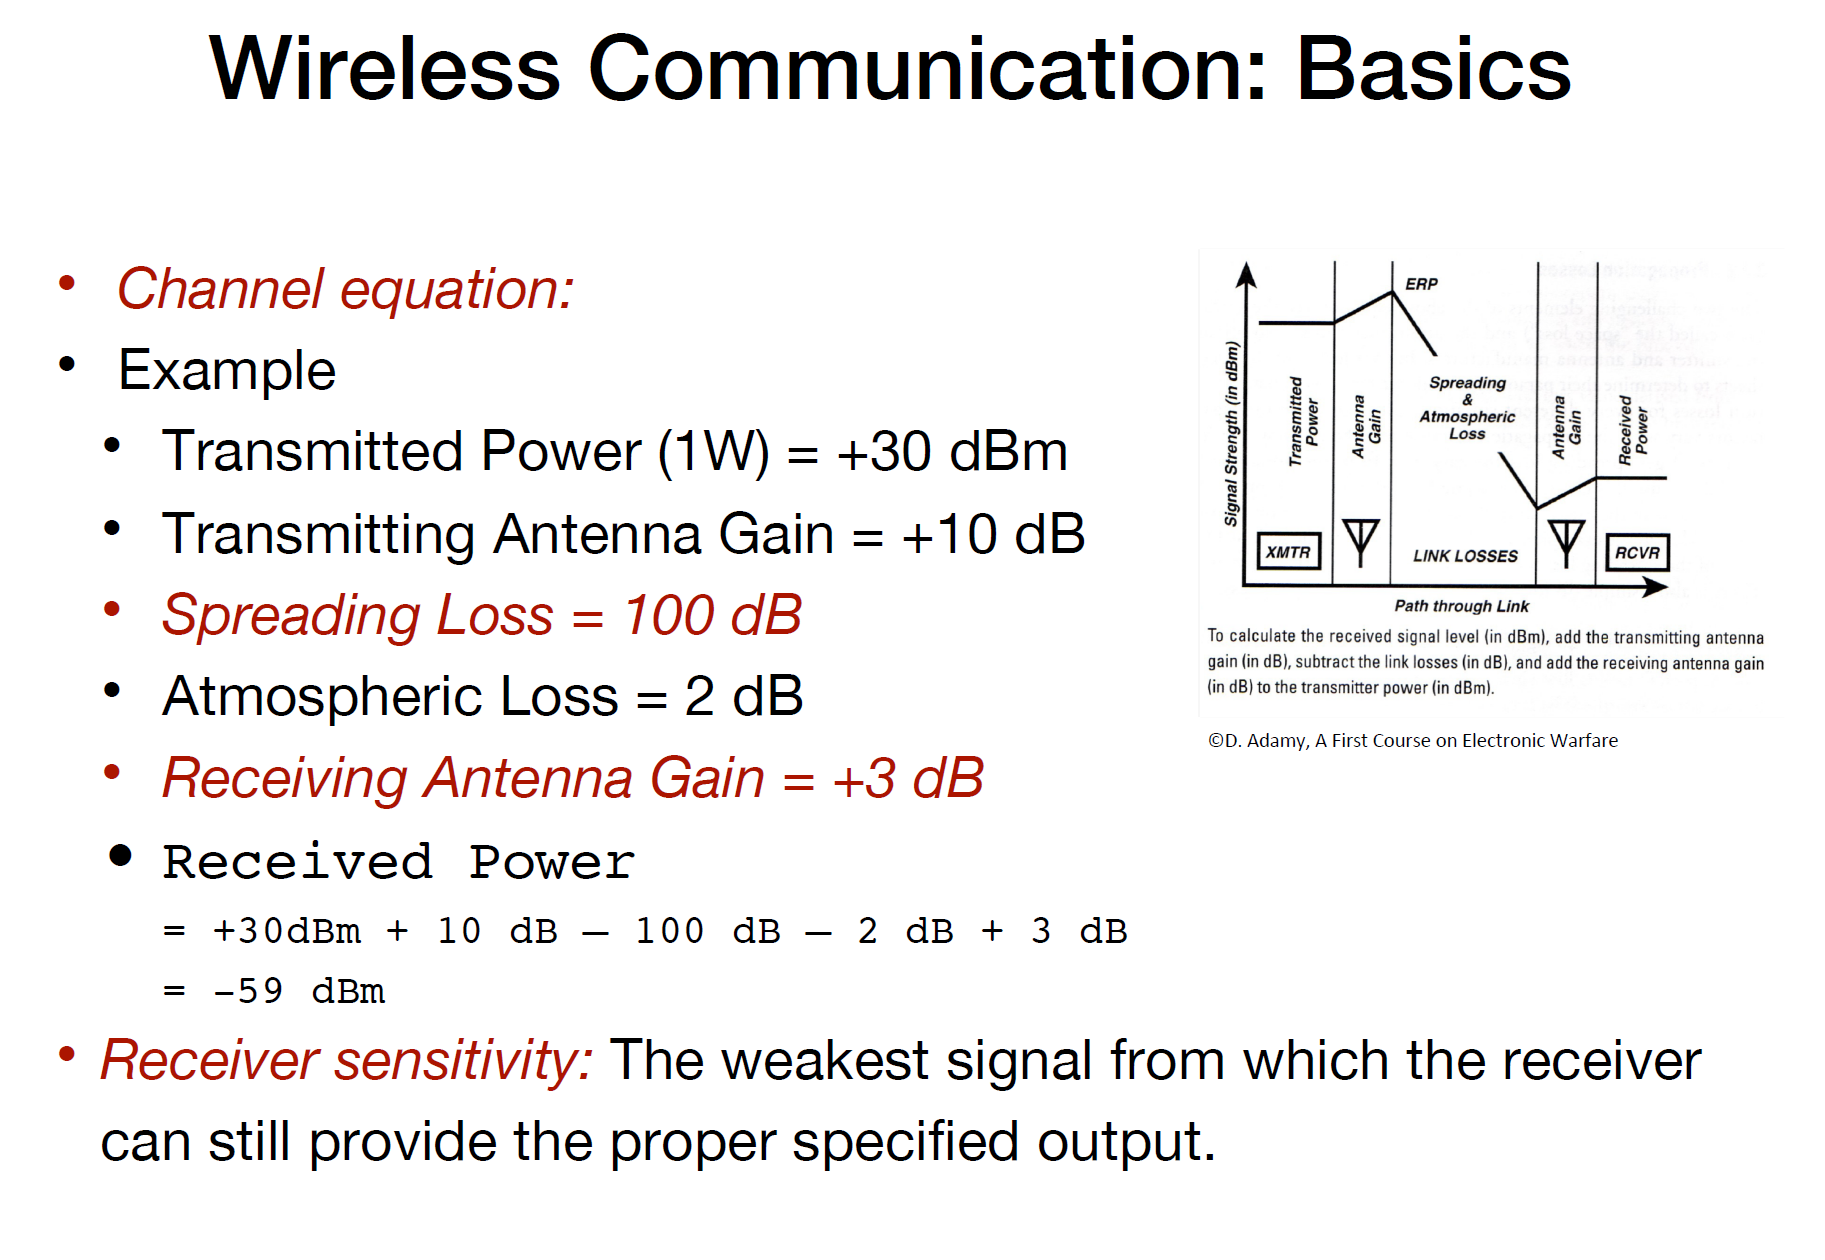
\includegraphics[width=\linewidth]{Figures/L1_channel_equation.PNG}
\end{minipage}

\begin{minipage}{\linewidth}
    \centering      
    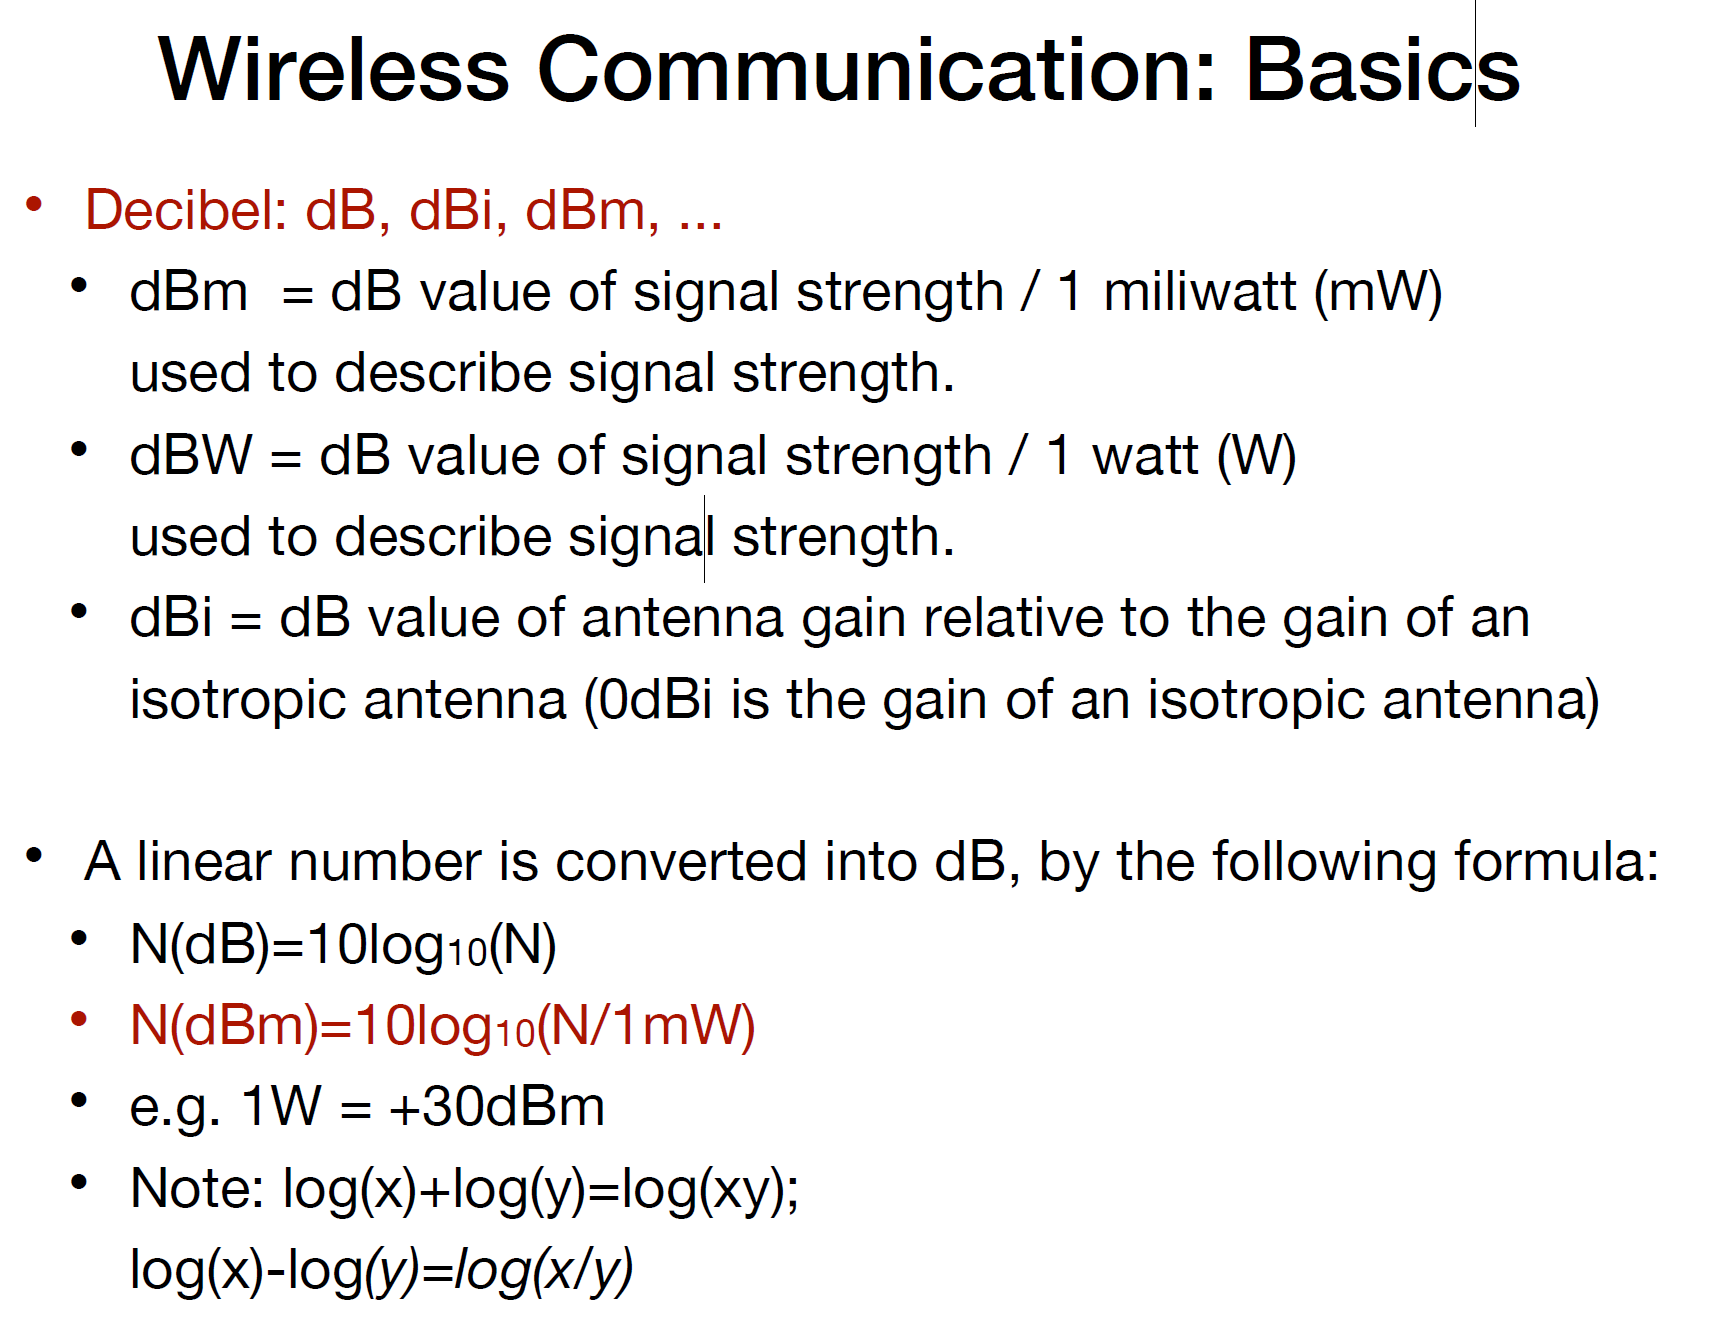
\includegraphics[width=\linewidth]{Figures/L1_signal_measures.PNG}
\end{minipage}

\subsection{Security}
Do we need Security in Wireless Networks?
\begin{itemize}
    \item We can't hide communication by disclosing carrier frequencies, as they can be discovered anyway by broadband receivers.
    \item We can't reach confidentiality through low power communication. Attacker with a good antenna might still pick up signal even though he is further away.
    \item Encryption, MAC/Signatures and new measures will help to increase security of wireless networks.
\end{itemize}
